\documentclass{beamer}
\usepackage[french]{babel}
\usepackage[T1]{fontenc}
\usepackage[utf8]{inputenc}

\usetheme{Frankfurt}

\title[Pr\'esentation du projet de ma\^itrise]{D\'eveloppement d'un module d'extension Moodle d'aide \`a la correction de questions\\de type \og texte long \fg{} }
\author{Philippe Girard}
\institute{Universit\'e du Qu\'ebec \`a Montr\'eal}
\date{26 juin 2018}

\begin{document}
  \begin{frame}[plain]
  \titlepage
  \end{frame}
  
  \begin{frame}[plain]
  \tableofcontents[hideallsubsections]
  \end{frame}
  
  \section[Introduction]{Motivation au projet}
  \begin{frame}
  \frametitle{Introduction au projet}
  Id\'ee de d\'epart:
  \begin{itemize}
    \item Par Guy Tremblay et Magda Fusaro
    \item Aide \`a la correction pour texte \`a d\'eveloppement
    \item Microsoft Word ou Moodle
  \end{itemize}
  \end{frame}
  
  \section[Moodle]{Introduction \`a Moodle et \`a son architecture modulaire}
  \begin{frame}
  \frametitle{\insertsection}
  \framesubtitle{Moodle}
  \begin{itemize}
    \item LMS (\textit{Learning Management System})
    \item Modulaire: Cours -> Sections -> Activit\'es
    \item Logiciel libre
  \end{itemize}
  \end{frame}
  
  \begin{frame}
  \frametitle{\insertsection}
  \framesubtitle{Les types de questions}
  Cr\'eation de formulaires en ligne
  
  \medskip
  
  Questions de types:
  \begin{itemize}
    \item Choix multiples
    \item R\'eponse courte
    \item Num\'erique
    \item Question Cloze
    \item Composition
  \end{itemize}
  \end{frame}
  
  \begin{frame}
  \frametitle{\insertsection}
  \framesubtitle{Les modules d'extensions Moodle}
  \begin{itemize}
    \item Rapport de questionnaire (\textit{Quiz report})
    \item Type de question (\textit{Question type})
    \item Comportement de question (\textit{Question behaviour})
  \end{itemize}
  \end{frame}
  
  \section[Mots-cl\'es]{D\'etection et analyse de mots-cl\'es}
  \begin{frame}
  \frametitle{\insertsection}
  \framesubtitle{La lemmatisation et la racination}
  La lemmatisation:
  \begin{itemize}
    \item Trouve le lemme
    \item Forme canonique d'un mot
    \item Aucune biblioth\`eque PHP fran\c{c}ais et anglais
  \end{itemize}
  
  \medskip
  
  La racination (\textit{stemming}):
  \begin{itemize}
    \item Trouve le radical (\textit{stem})
    \item Racine du mot
    \item Une biblioth\`eque multilingue PHP (\texttt{php-stemmer})
  \end{itemize}
  \end{frame}
  
  \begin{frame}
  \frametitle{\insertsection}
  \framesubtitle{Snowball}
  \texttt{php-stemmer} est une traduction PHP des algorithmes Snowball
  
  \bigskip
  
  Snowball:
  \begin{itemize}
    \item D\'evelopp\'e par Martin Porter
    \item Language de traitement de texte
    \item Compile en C ou en Java
    \item Algorithmes de racination pour 12 langues, dont le fran\c{c}ais
  \end{itemize}
  \end{frame}
  
  \section[Tests]{Tests pour int\'egration \`a Moodle d'un module d'extension}
  \begin{frame}
  \frametitle{\insertsection}
  \framesubtitle{Environnement de test}
  Machine virtuelle Xubuntu, PHP 7.0.22 et MySQL 5.7.20
  
  Moodle 3.4 install\'e avec Git
  \end{frame}
  
  \begin{frame}
  \frametitle{\insertsection}
  \framesubtitle{Tests unitaires}
  V\'erifications \`a petite \'echelle (m\'ethodes)
  
  D\'ependances remplac\'ees par des \textit{stubs}
  
  Ex\'ecut\'es avec \textit{PHPUnit}
  
  \bigskip
  
  8750 tests, 90 575 v\'erifications
  
  8682 \textit{success}, 67 \textit{skipped} et 1 \textit{failure}:
  \begin{itemize}
    \item Encodage de la base de donn\'ees UTF8 non sensible \`a la casse
  \end{itemize}
  \end{frame}
  
  \begin{frame}
  \frametitle{\insertsection}
  \framesubtitle{Tests d'acceptation}
  Tests automatis\'es, comme si un humain les ex\'ecutait
  
  Tests \textit{behat} ex\'ecut\'es avec \textit{Selenium}
  
  \bigskip
  
  1 771 sc\'enarios et 43 824 \'etapes
  
  4 sc\'enarios et 102 \'etapes ignor\'es
  
  6 sc\,énarios et 6 \'etapes \'echou\'es:
  \begin{itemize}
    \item Lorsqu'un \'etudiant passe d'une activit\'e \`a une autre
    \item Filtre du calendrier mensuel
    \item Navigation entre les modes de groupes
    \item Solr non install\'e (2 erreurs)
    \item L'enseignant ne voit pas quels \'etudiants sont actifs
  \end{itemize}
  \end{frame}
  
  \section[Mise en oeuvre]{Mise en oeuvre et tests du module d'extension \texttt{qtype\_essayhelper}}
  \begin{frame}
  \frametitle{\insertsection}
  \framesubtitle{Fonctionnalit\'es du module d'extension \texttt{qtype\_essayhelper}}
  Module d'extension bas\'e sur \texttt{qtype\_essay}
  
  Fonctionnalit\'es retir\'ees:
  \begin{itemize}
    \item \'Editeur de texte \textit{WYSIWIG}
    \item Remise de fichiers
  \end{itemize}
  
  Fonctionnalit\'es conserv\'ees:
  \begin{itemize}
    \item R\'etroaction g\'en\'erale
    \item Mod\`ele de r\'eponse
    \item Information de l'\'evaluateur
  \end{itemize}
  
  Fonctionnalit\'es ajout\'ees:
  \begin{itemize}
    \item Mots-cl\'es
    \item R\'eponse officielle de l'enseignant
    \item Langue de racination
  \end{itemize}
  \end{frame}
  
  \begin{frame}
  \frametitle{\insertsection}
  \framesubtitle{Structure des fichiers}
  \begin{center}
    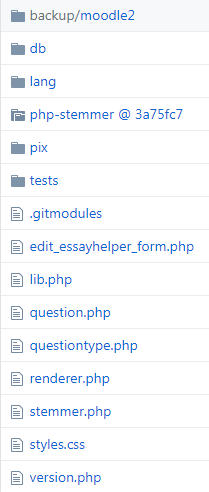
\includegraphics[scale=0.5]{../images/architecture.png}
  \end{center}
  \end{frame}
  
  \begin{frame}
  \frametitle{\insertsection}
  \framesubtitle{Principales classes}
  \begin{center}
    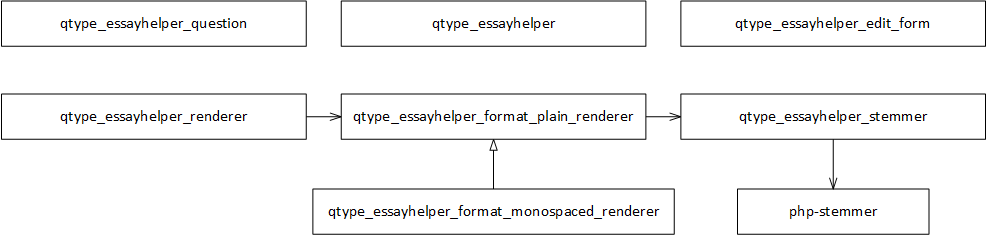
\includegraphics[scale=0.4]{../images/class-simple.png}
  \end{center}
  \end{frame}
  
  \section[R\'esultats]{R\'esultats obtenus et limites de notre module de correction}
  \begin{frame}
  \frametitle{\insertsection}
  \framesubtitle{Exemple de configuration}
  \begin{center}
    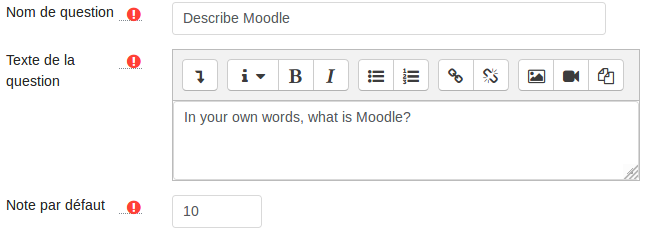
\includegraphics[scale=0.4]{../images/questionform_base.png}
    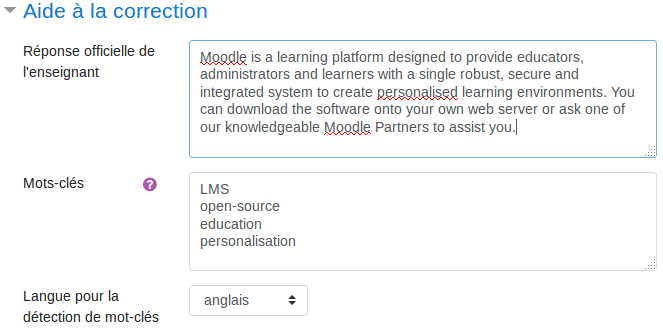
\includegraphics[scale=0.4]{../images/questionform_helper.png}
  \end{center}
  \end{frame}
  
  \begin{frame}
  \frametitle{\insertsection}
  \framesubtitle{Exemple d'interface de correction}
  \begin{center}
    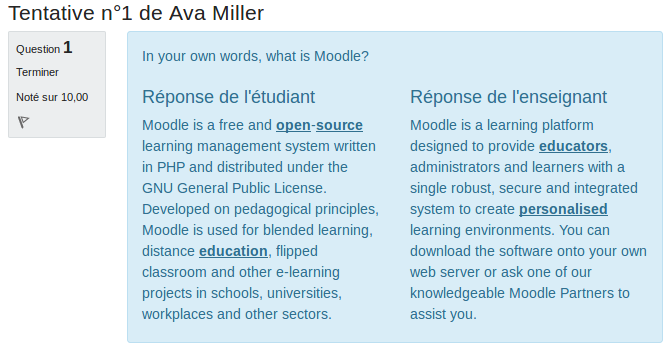
\includegraphics[scale=0.4]{../images/questionform_correction.png}
  \end{center}
  \end{frame}
  
  \begin{frame}
  \frametitle{\insertsection}
  \framesubtitle{Limites du projet 1/2}
  Pas de tests réels:
  \begin{itemize}
    \item Professeure Fusaro est devenue Rectrice de l'UQAM
    \item Les \'evaluations dans mes cours n'ont pas de textes \`a d\'eveloppement
  \end{itemize}
  
  \bigskip
  
  La s\'eparation des mots est probl\'ematique:
  \begin{itemize}
    \item \og aujourd'hui \fg{} devient \og aujourd \fg{} et \og hui \fg{} 
    \item \og qu'autrui \fg{} devient \og qu \fg{} et \og autrui \fg{} 
    \item \og wasn't \fg{} devient \og wasn \fg{} et \og t \fg{} 
  \end{itemize}
  \end{frame}
  
  \begin{frame}
  \frametitle{\insertsection}
  \framesubtitle{Limites du projet 2/2}
  Certains mots cl\'es peuvent \^etre mis en \'evidence plusieurs fois:
  \begin{itemize}
    \item \og aimera \fg{} accompagn\'e de \og aimerait \fg{} avec mot-cl\'e \og aimer \fg{}
  \end{itemize}
  \end{frame}
  
  \begin{frame}
  \frametitle{\insertsection}
  \framesubtitle{Am\'eliorations possibles}
  Mise en \'evidence configurable via l'interface
  
  Utilisation de la lemmatisation
  
  Comparaison des r\'eponses des \'etudiants pour plagiat
  \end{frame}
  \section[Conclusion]{Conclusion}
  \begin{frame}
  \frametitle{\insertsection}
  Mise en pratique de nouveaux outils:
  \begin{itemize}
    \item Tests unitaires
    \item Tests d'acceptation
    \item \LaTeX
  \end{itemize}
  
  Apprentissages:
  \begin{itemize}
    \item Analyser avant de se lancer
    \item G\'erer mon horaire
    \item \'Ecrire des rapports et des notes de cours
  \end{itemize}
  \end{frame}
  
  \begin{frame}
  \begin{center}
  \Huge Questions?
  \end{center}
  \end{frame}
\end{document}